\section{\index{SiC!Silicon Carbide}{Silicon Carbide}}\label{SiC}
\todo[color=red, inline]{Check wrapfigs}

\index{SiC}{SiC} is considered an excellent semiconductor material for high-power, high-temperature, and high-frequency electronics \cite{Eddy2009,CASADY19961409}. Studies have demonstrated SiC's potential as a host material for qubits, which enables the development of quantum sensors. 



A qubit system is, in the simplest terms, as a two-level system. The power of a \index{qubit}{qubit} lies in quantum coherence and/or
temporal superposition of quantum states which allow for computation or manipulation with no classical analogue before being collapsed back to a measurement basis. 



\subsection{Defects}

% \begin{figure}[!htb]
\begin{figure}[H]
    \begin{center}
        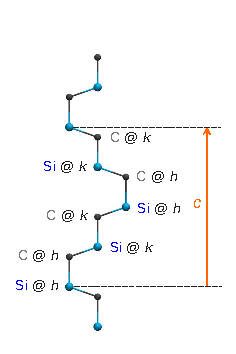
\includegraphics[width=0.32\textwidth]{figures/SiC-non-equiv-sites.pdf}
        \hspace{1em}
        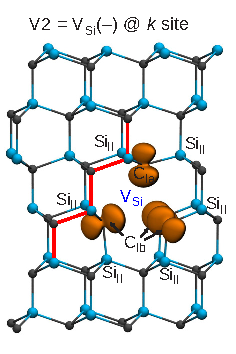
\includegraphics[width=0.32\textwidth]{figures/SiC-V2.pdf}
    \end{center}
    \caption{}\label{fig:}
\end{figure}


\subsubsection{$S=1$ Defects}

% \begin{wrapfigure}{r}{0.4\textwidth}%
%     \centering%
%     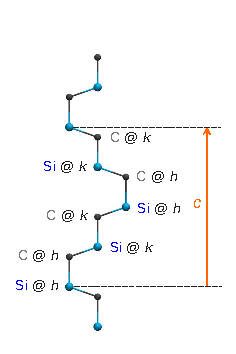
\includegraphics[width=0.38\textwidth]{figures/SiC-non-equiv-sites.pdf}%
%   \caption{C-axis and non-equiv sites in 4H SiC \td{better caption}}%
% \end{wrapfigure}%


\subsubsection{$S=3/2$ Defects}


% \begin{wrapfigure}{l}{0.36\textwidth}%
%     \centering%
%     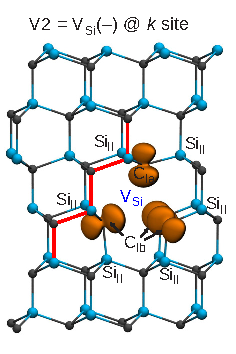
\includegraphics[width=0.34\textwidth]{figures/SiC-V2.pdf}%
%   \caption{ \td{better caption}}%
% \td{ensure wrapfigs aligned before final submission - no white space onto subsequent page}
% \end{wrapfigure}%




% large-area, high-quality SiC substrates readily available for applications such as high-frequency transmitters and solid-state white lighting
\cite{Eddy2009}


% has emerged as the most mature of the wide-bandgap (2.0 eV ≲ Eg ≲ 7.0 eV) semiconductors
\cite{CASADY19961409}


% Here, we present the coherent manipulation of single divacancy spins in 4H-SiC with a high readout contrast (⁠⁠) and a high photon count rate (150 kilo counts per second) under ambient conditions, which are competitive with the nitrogen-vacancy centres in diamond. 
\cite{10.1093/nsr/nwab122}


% Point defects in wide-bandgap semiconductors can have both ground and excited states within the energy gap and, hence, are luminescent centers or often called color centers. With the ground state being deep in the bandgap, the luminescence is often stable even at room temperature. Many color centers also possess a non-zero electron spin and can be excellent candidates for optical spin quantum bits (qubits).
\cite{Son2021}

% silicon vacancy in an industry-friendly platform, SiC, has the potential for various magnetometry applications under ambient conditions.
\cite{PhysRevApplied.6.034001}

% Silicon carbide is an emerging platform for quantum technologies that provides wafer scale and low-cost industrial fabrication.
\cite{Jiang2023}

% Although NV centers in diamond have shown remarkable spin properties, diamond as a host material is not compatible with conventional electronic circuits (14). By comparison, silicon carbide (SiC) is a technology-friendly material with a large-scale production capacity and mature doping techniques
\cite{Jiang2023}


% SiC is a transparent material from the UV to the infrared, possess nonlinear optical properties from the visible to the mid-infrared and it is a meta-material in the mid-infrared range. SiC fluorescence due to color centers can be associated with single photon emitters and can be used as spin qubits for quantum computation and communication networks and quantum sensing. This unique combination of excellent electronic, photonic and spintronic properties has prompted research to develop novel devices and sensors in the quantum technology domain.
\cite{Castelletto2022}


% current applications in single-photon sources, quantum sensing of strain, magnetic and electric fields, spin-photon interface are also described. Finally, the efforts in the integration of these color centers in photonics devices and their fabrication challenges are described.
\cite{Castelletto2020-ie}


\subsection{Production of $\ce{SiC}$}
%  electrical properties of SiC, which outstand
% the host material of the NV centers, and the mature fab-
% rication technology, which allows an efficient fabrication
% of electronic devices even at the atomic scale
\cite{arxiv.1503.07566}

% The on-demand engineering of optically active spins in technologically friendly materials is a crucial step toward implementation of both maser amplifiers, requiring high-density spin ensembles, and qubits based on single spins. 
\cite{Fuchs2015}


% we discuss energetic particle irradiation, especially proton beam writing (PBW), in which proton microbeams with MeV range are used, as a method to create VSi in SiC since PBW can create VSi in certain locations with micrometer accuracy and this is very useful to introduce VSi in electronic devices without the degradation of their electrical characteristics.
\cite{Ohshima2018}

% Finally, we show the successful generation and characterization of single nitrogen vacancy (NV) center in SiC employing ion implantation. 
\cite{Mu2020}


 % we present the generation and characterization of shallow silicon vacancies in silicon carbide by using different implanted ions and annealing conditions. 
\cite{Wang2019}


% Here, we demonstrate a scalable approach of manufacturing solid-immersion lenses (SILs) on 4H–SiC.
\cite{Sardi2020}

\subsection{Colour Defects in $\ce{SiC}$}
\begin{figure}[h]
    \begin{center}
        % \includegraphics[width=0.95\textwidth]{figures/}
        \missingfigure{Diagram of possible SiC defects showing orientation/position within the lattice}
    \end{center}
    \caption{}\label{fig:}
\end{figure}

\subsubsection{Electronic Structure}
\subsubsection{Charge State}
\subsubsection{Spin System}




